\chapter{Statistical machine learning and convex optimization by
\href{https://www.di.ens.fr/~fbach/}{Francis Bach}}
%\newrefsection

\section{Introduction 14:30--18:00}

We will use $n$ for the number of observations and $d$ for de dimension size.
When working with big data we will seek ideally for a running-time complexity
of $O(dn)$.


\section{Classical methods for convex optimization}

In supervised learning we have a set of observations $(x_i, y_i) \in X, Y,
i=1,\dots,n$, i.i.d. (this assumption is almost never true).

For regression $y \in \Real$ and prediction $\hat{y} = \theta^T \Phi(x)$, for
classification $y \in {-1, 1}$ and the prediction is $\hat{y} =
\text{sign}(\theta^T \Phi(x))$.

Empirical risk minimization to find a $\hat{\theta}$ solution to

\begin{equation}
  \argmin_{\theta \in \Real^d} 1/n \sum_{i=1}^n l(y_i, \theta^T \Phi(x_i)) +
    \mu \Omega(\theta)
\end{equation}

the training cost (or empirical risk) is

\begin{equation}
  \hat{f}(\theta) = 1/n \sum_{i=1}^n l(y_i, \theta^T \Phi(x_i))
\end{equation}

and the testing cost or expected risk is

\begin{equation}
  \hat{f}(\theta) = \Expected_{(x,y)}l(y_i, \theta^T \Phi(x_i))
\end{equation}

This imposes two fundamental questions: (1) how are we finding the optimal set
of parameters $\theta$ and (2) how to analyse $\hat{\theta}$.

The loss for a single observation is $f_i(\theta) = l(y_i, \dots$ TODO missing

Jensen inequality says that $g(\Expected(\theta) \le \Expected g(\theta)$

The global definition of convexity if we assume differrntiability is

\begin{equation}
  \forall \theta_1, \theta_2, g(\theta_1) \le g(\theta_2) + g'(\theta_2)^T(\theta_1 - \theta_2)
\end{equation}

With twice differentiable functions $\forall \theta, g''(\theta) \succeq 0$
(positive semi-definite Hessians).

We ideally want a convex problem because the local minimum is the same as the
global minimum, with an optimal condition in $g'(\theta) = 0$. See also the convex
duality and recognizing convex problems in \cite{boyd2004convex}.

\subsection{Lipschitz continuity}

Bounded gradients of g (lipschitz-continuity) if the function g is convex,
differentiable and has a

\subsection{Smoothness and strong convexity}

\begin{theorem}
  A function $g : \Real^d \ra \Real$ is \emph{L-smooth} if and only if it is
  differentiable and its gradient is L-Lipschitz-continuous
  \begin{equation}
    \forall \theta_1, \theta_2 \in \Real^d, ||g'(\theta_1) - g'(\theta_2) ||_2
    \le L||\theta_1 - \theta_2||_2
  \end{equation}
\end{theorem}

Adding a regularization $\mu/2 ||\theta||^2$ with a value of $\mu$ on the order
of $1/n$.

\subsection{Analysis of empirical risk minimization}

most important slide from the first part is summarized in slide 47


\subsection{Accelerated gradient methods (Nesterov, 1983)}

Algorithm

\begin{align}
  \theta_t = \eta_{t-1} - \frac{1}{L}g'(\eta_{t-1}) \\
  \eta_t = \theta_t + \frac{t-1}{t+2}(\theta_t - \theta_{t-1})
\end{align}

with bound

\begin{equation}
  g(\theta_t) - g(\theta_*) \le \frac{2L ||\theta_0 - \theta_*||^2}{(t+1)^2}
\end{equation}

\subsection{Optimization fro sparsity-inducing norms}

See Bach, Jenatton, Mairal, and Obozinski, 2012b \cite{bach2012optimization}.

\subsubsection{Newton method}

Minimize the  second-order Taylor expansion


\subsection{Summary about minimization of convex functions}

\begin{itemize}
  \item Gradient descent: $\theta_t = \theta_{t-1}- \gamma_t g'(\theta_{t-1})$
    \begin{itemize}
      \item $O(1/\sqrt{t})$ convergence rate for non-smooth convex functions
      \item $O(1/t)$ convergence rate for smooth convex functions
      \item $O(e^{-pt})$ convergence rate for strongly smooth convex functions
    \end{itemize}
  \item Newton method: $\theta_t = \theta_{t-1}- g''(\theta_{t-1})^{-1}g'(\theta_{t-1})$
    \begin{itemize}
      \item $O(e^{-p2^t})$ convergence rate
    \end{itemize}
  \item Key insights from Bottou and Bousquet (2008)
    \begin{itemize}
      \item In machine learning, it is not necessary to optimize below
        statistical error
      \item In machine learning the cost functions are averages
      \item Testing errors are more important than training errors
    \end{itemize}
\end{itemize}

\section{Convex stochastic approximation}

There are known global minimax? rates of convergence for non-smooth problems
(Nemirovsky and Yudin, 1983; Agarwal et al., 2012).


\begin{itemize}
  \item Least-squares regression is easy to analyze, and has an explicit
    relationship to bias/variance trade-offs (see Défossez and Bach (2015);
      Dieuleveut et al. (2016).
  \item Many important loss functions are not quadratic (see Bach and Moulines
    (2013)).
\end{itemize}

\begin{figure}[h]
  \centering
  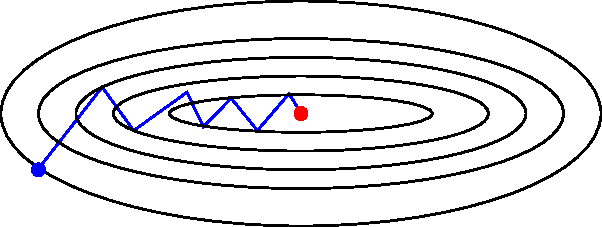
\includegraphics[width=.5\textwidth]{figures/optimization/optimization_batch_gd}
  \caption{Batch Gradient Descent: it needs to decrease the error on every
  step, if not, then the parameters are not right}
\end{figure}

\begin{figure}[h]
  \centering
  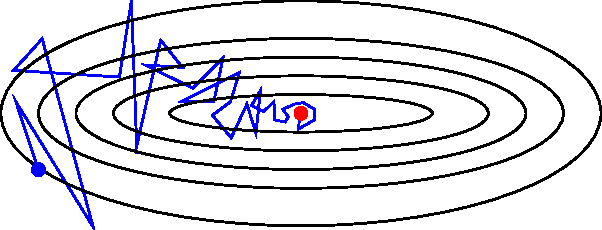
\includegraphics[width=.5\textwidth]{figures/optimization/optimization_stochastic_gd}
  \caption{Stochastic Gradient Descent: the error may increase ocasionally}
\end{figure}

\section{Summary of rates of convergence}

Given the problem parameters

\begin{itemize}
  \item $D$: diameter of the domain
  \item $B$ Lipschitz-constant
  \item $L$ smoothnesss constant
  \item $\mu$ strong convexity constant
\end{itemize}


\begin{table}[h]
  \def\arraystretch{1.4}
  \centering
  \begin{tabular}{|c|c|c|}
    \hline
    & \textbf{convex} & \textbf{strongly convex} \\
    \hline
    nonsmooth & deterministic: $BD/\sqrt{t}$ & deterministic: $B^2/(t\mu)$ \\
              & stochastic: $BD/\sqrt{n}$ & stochastic: $B^2/(n\mu)$ \\
    \hline
    smooth & deterministic: $LD^2/t^2$ & deterministic: $\exp(-t\sqrt{\mu/L})$ \\
           & stochastic: $LD^2/\sqrt{n}$ & stochastic: $L/(n\mu)$ \\
           & finite sum: $n/t$ & finite sum: $\exp(-t/(n+L/\mu))$ \\
    \hline
    quadratic & deterministic: $LD^2/t^2$ & deterministic: $\exp(-t\sqrt{\mu/L})$ \\
              & stochastic: $d/n + LD^2/n$ & stochastic: $d/n + LD^2/n$ \\
    \hline
  \end{tabular}
  \caption{Summary of rates of convergence}
\end{table}

\section{Conclusions}

\begin{itemize}
  \item Statistics with our without optimization
    \begin{itemize}
      \item Significance of mixing algorithms with analysis
      \item Benefits of mixing algorithms with analysis
    \end{itemize}
  \item Open problems
    \begin{itemize}
      \item Non-parametric stochastic approximation (Dieuleveut and Bach, 2014)
      \item Characterization of implicit regularization of online methods
      item Structured prediction
      \item Going beyond a single pass over the data (/testint performance)
      \item Parallel and distributed optimization
      \item Non-convex optimization (Reddi et al., 2016)
    \end{itemize}
\end{itemize}
